\documentclass[10pt,twocolumn]{article}

\usepackage[letterpaper,margin=0.72in,columnsep=0.25in]{geometry}
\usepackage[T1]{fontenc}
\usepackage[utf8]{inputenc}
\usepackage{lmodern}
\usepackage{microtype}
\usepackage{amsmath,amssymb}
\usepackage{booktabs}
\usepackage{tabularx}
\usepackage{graphicx}
\usepackage{caption}
\usepackage{subcaption}
\usepackage{enumitem}
\usepackage[dvipsnames]{xcolor}
\usepackage[round,authoryear]{natbib}
\usepackage[hidelinks]{hyperref}
\usepackage{url}

\graphicspath{{../artifacts/figures/}}
\setlength{\parindent}{1em}
\setlength{\parskip}{0pt}
\setlist{nosep,leftmargin=*}
\captionsetup{font=small,labelfont=bf}
\renewcommand{\arraystretch}{1.08}
\title{Robustness of Text Classification to Adversarial Unicode Perturbations:\\A Comparative Study of Word-, Character-, and Subword-Based Representations}
\author{Lorenzo Marinelli (2043092)\\Sapienza University of Rome}
\date{Academic Year 2025--2026}

\begin{document}
\maketitle

\begin{abstract}
Text classifiers receive Unicode strings, while readers primarily perceive rendered glyphs. This mismatch enables adversarial changes that preserve the apparent text but alter its code points and tokenization. We compare word and character TF--IDF classifiers, an \texttt{o200k\_base} BPE-feature classifier, and fine-tuned DistilBERT on BANKING77 intent detection and coarse TREC question classification. The evaluation covers homoglyph substitutions, invisible characters, compatibility characters, canonical composition, and mixed attacks at four strengths. We additionally evaluate Unicode normalization, removal of default-ignorable characters, and an English-specific confusable-repair heuristic. Beyond accuracy and Macro-F1, we measure attack success, defense recovery, token-sequence disruption, and the association between tokenization changes and failures. The resulting study separates controlled representation effects from the behavior of a pretrained Transformer and identifies both the value and the limits of low-cost input sanitization.
\end{abstract}


\section{Introduction}

Text classification is commonly formulated as a mapping $f(x)=y$ from a Unicode string $x$ to a discrete label $y$. For an intent detector, ``How can I reset my PIN?'' should map to a password or PIN-related intent. A user can, however, replace Latin \texttt{a} (U+0061) with Cyrillic small letter a (U+0430), insert a zero-width character, use a compatibility form, or change canonical composition. The rendered utterance can remain indistinguishable or nearly indistinguishable while the classifier receives a different sequence of code points.

This is a practical concern for intent classification, spam and phishing filters, content moderation, and other systems exposed to untrusted text. It is also a useful scientific setting: word, character, and subword representations transform the same perturbation in different ways. A word vocabulary may turn one modified character into an out-of-vocabulary token; character $n$-grams may lose only local features; and byte-pair or WordPiece tokenizers may fragment one familiar word into several uncommon tokens.

We address four questions:
\begin{enumerate}
  \item How does classification degrade as the perturbation rate increases?
  \item Are word-, character-, BPE-, and Transformer-based systems affected differently?
  \item Are subword tokenization changes associated with attack success?
  \item Can lightweight Unicode preprocessing recover attacked performance without harming clean inputs?
\end{enumerate}

The central comparison holds the downstream classical classifier fixed: three TF--IDF representations feed Logistic Regression. DistilBERT is included as a modern pretrained reference rather than as a controlled representation-only comparison. All models receive exactly the same attacked examples.

The contribution is a reproducible experiment rather than a new attack algorithm. It combines (i) a shared, auditable attack corpus with gradual budgets and three attack seeds; (ii) a controlled comparison of word, character, and BPE features; (iii) a pretrained Transformer reference with three fine-tuning seeds; (iv) deployment-style defenses applied to both clean and attacked inputs; and (v) paired uncertainty and tokenization diagnostics. This design makes it possible to distinguish an attack's nominal strength from its effective coverage and to ask whether a defense restores performance at the cost of changing legitimate clean text.

\section{Related Work}

\citet{eger2019visual} show that visually similar character substitutions substantially damage neural and non-neural NLP systems across character-, word-, and sentence-level tasks. They also study visual embeddings, adversarial training, and rule-based recovery. \citet{boucher2022bad} broaden the threat model to imperceptible encoding-level attacks, including invisible characters, homoglyphs, reorderings, and deletion controls, and demonstrate black-box failures in deployed and open-source systems.

Both studies motivate a representation-level comparison, but their scope is broader than the present controlled classification setting. Eger et al.\ provide VIPER attack and shielding code, while Boucher et al.\ provide generators and detectors for encoding perturbations. Here, those ideas are narrowed to auditable, single-code-point transformations with fixed budgets so every classifier can be evaluated on identical rows.

Tokenization provides a complementary explanation. \citet{chai2024tokenization} analyze subword sensitivity to typographical and formatting variation and show that larger models do not eliminate the problem. \citet{geh2025adversarial} manipulate the selection of valid token sequences without changing the visible input. Their attack is not a Unicode perturbation, but it establishes tokenization itself as a security-relevant interface.

Chai et al.\ release their TKEval code and data and report that regularized tokenization can improve resilience. Geh et al.\ instead exploit alternative valid segmentations at the model interface; this is adjacent tokenization-security work, not evidence about Unicode homoglyphs. Our token edit, count, and overlap measurements connect encoding perturbations to failures without conflating these distinct threat models.

For defenses, \citet{cooper2025lies} use proprietary and open-source language models to normalize homoglyph-obfuscated text. Our focus is deliberately cheaper: deterministic normalization, removal of default-ignorable characters, and a restricted confusable map. Unicode normalization has precise equivalence guarantees, but NFKC can erase meaningful compatibility distinctions \citep{unicode15}. Likewise, confusable skeletons are intended for security analysis rather than arbitrary display-text replacement \citep{unicode39}. We therefore measure clean-text harm and present confusable repair as an English-specific heuristic.

Cooper et al.\ release code and an augmented tweet dataset, enabling comparison with more flexible but more expensive normalization. Our experiment does not claim state of the art across all adversarial text defenses. Instead, it establishes transparent low-cost baselines whose transformations can be inspected code point by code point and whose clean-input behavior can be measured directly.

\section{Comparative evaluation}
\subsection{The four different text representations}
The classical models share Logistic Regression, the data split and validation. Vocabulary sizes and feature geometry still differ because the representations work differently: for example, a single word produces several character $n$-grams. DistilBERT \cite{sanh2019distilbert} has a different architecture, so it serves as a separate reference.

\begin{center}
\begin{minipage}{\linewidth}
\centering\small
\captionof{table}{Model input representations.}
\begin{tabularx}{\linewidth}{@{}L{0.27\linewidth}Y@{}}
\toprule
\tabhead Model & Input representation \\
\midrule
Word TF--IDF & Word unigrams and bigrams. \\
Character TF--IDF & Character 3--5-grams. \\
BPE TF--IDF & \texttt{o200k\_base} token-ID unigrams and bigrams. \\
DistilBERT & Uncased WordPiece; maximum 128 tokens. \\
\bottomrule
\end{tabularx}
\end{minipage}
\end{center}

For all three TF--IDF models, I chose \(C\in\{0.1,1,10\}\) by validation Macro-F1; each selected \(C=10\) on both datasets. DistilBERT used three epochs, a learning rate of \(2\times10^{-5}\), effective batch size 16, weight decay 0.01 and warmup ratio 0.10.

\subsection{What changes in an attacked input?}
Each attack samples eligible positions reproducibly, then the clean and attacked examples gets stored together with the edits made.

\begin{center}
\begin{minipage}{\linewidth}
\centering\small
\captionof{table}{Attack families and where they apply.}
\begin{tabularx}{\linewidth}{@{}L{0.29\linewidth}Y@{}}
\toprule
\tabhead Family & Transformation and eligibility \\
\midrule
Homoglyph & Replace mapped letters with curated Greek or Cyrillic lookalikes. \\
Invisible & Insert a default-ignorable control after an alphanumeric character. \\
Compatibility & Use alternate forms whose NFKC normalization recovers the source. \\
Composition & Decompose a precomposed character when it has a canonical decomposition. \\
Mixed & At each eligible position, sample one applicable transformation. \\
\bottomrule
\end{tabularx}
\end{minipage}
\end{center}

The attack strengths tested are 5\%, 10\%, 20\%, 40\% and 75\% of eligible positions.

\subsection{Coverage of the methods}
A nominal budget is meaningful only if the attack can effectively change the text samples. The four broad families reach every test example at 20\% (I'll take this as the main strength from now on); canonical composition reaches none (Table~\ref{tab:coverage}). Its unchanged test score therefore provides no evidence of robustness, because no test input has an eligible canonical decomposition. Naturally accented text could give a different result.

\begin{center}
\begin{minipage}{\linewidth}
\centering\small\setlength{\tabcolsep}{3pt}
\captionof{table}{Coverage and average edits per example at 20\% strength. B77 denotes BANKING77.}
\begin{tabular}{lrrrr}
\toprule
Attack & B77 cov. & B77 changes & TREC cov. & TREC changes \\
\midrule
homoglyph & 1.00 & 4.86 & 1.00 & 3.26 \\
invisible & 1.00 & 8.54 & 1.00 & 5.64 \\
compatibility & 1.00 & 8.85 & 1.00 & 5.88 \\
composition & 0.00 & 0.00 & 0.00 & 0.00 \\
mixed & 1.00 & 8.85 & 1.00 & 5.88 \\
\bottomrule
\end{tabular}

\label{tab:coverage}
\end{minipage}
\end{center}

Budgets are relative to each family's eligible positions so the same percentage does not produce the same number of edits for different attack kinds. 

\subsection{Five test-time defenses}
The models are evaluated without retraining. Each wrapper processes both clean and attacked inputs, making any clean-text harm visible. NFC and NFKC follow Unicode normalization rules; neither is a general solution to cross-script lookalikes \cite{unicode15,unicode39}.

\begin{table*}[!tbp]
\centering\small
\caption{Defense scope. ``Full repair'' names the most complete wrapper in this experiment.}
\begin{tabularx}{\linewidth}{@{}L{1.35in}Y Y@{}}
\toprule
\tabhead Wrapper & Operation & Intended coverage \\
\midrule
NFC & Canonical composition. & Canonical equivalence; untested here because composition coverage is zero. \\
NFKC & Compatibility normalization. & The generated compatibility substitutions. \\
Control removal & Remove default-ignorable characters. & The selected invisible insertions. \\
NFKC + removal & Apply both operations in sequence. & Compatibility and invisible changes. \\
Full repair & Add restricted non-ASCII-to-ASCII confusable repair. & Also the curated homoglyphs; assumes English/ASCII targets. \\
\bottomrule
\end{tabularx}
\end{table*}


\subsection{How the result measures work}
\label{sec:measures}
Let \(N\) be the number of test examples and \(K\) the number of classes. For class \(k\), \(TP_k\) counts correct predictions of that class, \(FP_k\) counts incorrect predictions of it, and \(FN_k\) counts its missed examples.


\minisection{Accuracy} Correct predictions divided by \(N\); each example has equal weight.

\minisection{Macro-F1} Precision and recall are balanced within each class, then all classes have equal weight:
\[
M=\frac{1}{K}\sum_{k=1}^{K}\frac{2TP_k}{2TP_k+FP_k+FN_k}.
\]
From now on, \(M\) denotes Macro-F1. A class with no correct predictions receives F1 zero. Accuracy weights frequent classes more heavily, while Macro-F1 prevents them from dominating the average. That's why it is useful in these multiclass classification tasks.

\minisection{Macro-F1 loss} \(M_{\mathrm{raw,clean}}-M_{\mathrm{raw,attacked}}\). A loss of 0.10 is ten F1 percentage points, not a 10\% relative loss. 

\minisection{Attack success rate (ASR)} Newly incorrect examples divided by examples correct when clean. It measures how often an attack overturns an initially correct prediction; baseline errors are excluded. ASR is undefined if no examples are correct when clean. For example: if 80 of 100 examples are correct when clean and an attack overturns 20 of those 80 predictions, ASR is \(20/80=25\%\). It is not the attacked error rate: the 20 original errors are outside its denominator, and some of those could become correct after attack (which would be by sheer luck and it's not worth investigating in the current study).


\minisection{Clean-score delta} \(M_{\mathrm{defended,clean}}-M_{\mathrm{raw,clean}}\). A negative value means that the wrapper harms clean performance.



\subsection{Defense recovery \texorpdfstring{\(R\)}{R}}
\label{sec:recovery-definition}
Recovery measures the fraction of the attack-induced Macro-F1 loss that a wrapper restores:
\begin{equation}
R=\frac{M_{\mathrm{defended,attacked}}-M_{\mathrm{raw,attacked}}}
        {M_{\mathrm{raw,clean}}-M_{\mathrm{raw,attacked}}}.
\label{eq:recovery}
\end{equation}

If \(R=0\), the attacked score is unchanged; \(R=0.5\) means half of the lost Macro-F1 is recovered; and \(R=1\) means the clean baseline is reached. Values are not clipped so repair can make the score worse (\(R<0\)) or raise it above the clean baseline (\(R>1\)), lastly Recovery is undefined when the raw attack causes no positive loss.

For each condition, I calculate the metrics on the matched test examples, but to keep tidyness and avoid entire pages of only tables for some of them I averaged the scores of the different attacks families. The overall attacked score gives equal weight to homoglyph, invisible, compatibility and mixed attacks. Composition is excluded from that average because it changes no inputs.

\subsection{Results}
To keep the presentation clear, tables and plots show mean scores without standard-deviation annotations.
\begin{center}
\begin{minipage}{\linewidth}
\centering
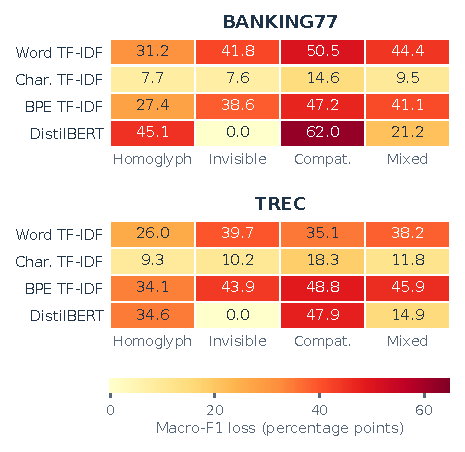
\includegraphics[width=\linewidth]{attack_family_comparison.pdf}
\captionof{figure}{Macro-F1 loss at 20\% strength, without defenses (larger is worse). Mixed is not always the hardest attack: on BANKING77, DistilBERT loses 62.0 points to compatibility changes, 21.2 to mixed attacks and none to invisible controls. Composition is omitted because it changes no inputs.}
\label{fig:attack-family-comparison}
\end{minipage}
\end{center}

\minisection{Clean accuracy does not settle the robustness comparison}
Character TF--IDF has the strongest clean BANKING77 score, while DistilBERT leads on TREC. At the main 20\% strength setting, character features retain the highest average Macro-F1 on both datasets (Table~\ref{tab:performance}). Their attack-success rates are also the lowest: fewer initially correct predictions are overturned.

\begin{table*}[!tbp]
\centering\small
\caption{Clean and attacked test performance. Attacked F1, loss and ASR average the four effective families at 20\%.}
\begin{tabular}{@{}lrrrrr@{}}
\toprule
\tabhead Model & Clean acc. & Clean F1 & Attacked F1 & F1 loss & ASR \\
\midrule
\multicolumn{6}{l}{\textbf{BANKING77}} \\
Word TF-IDF & 0.885 & 0.886 & 0.466 & 0.420 & 49.0\% \\
Character TF-IDF & 0.906 & 0.906 & 0.807 & 0.099 & 12.5\% \\
BPE TF-IDF & 0.882 & 0.882 & 0.496 & 0.386 & 45.3\% \\
DistilBERT & 0.832 & 0.819 & 0.498 & 0.321 & 40.8\% \\
\addlinespace[5pt]
\multicolumn{6}{l}{\textbf{TREC}} \\
Word TF-IDF & 0.888 & 0.885 & 0.537 & 0.347 & 38.6\% \\
Character TF-IDF & 0.888 & 0.883 & 0.759 & 0.124 & 17.9\% \\
BPE TF-IDF & 0.890 & 0.879 & 0.447 & 0.432 & 45.4\% \\
DistilBERT & 0.967 & 0.944 & 0.701 & 0.243 & 27.4\% \\
\bottomrule
\end{tabular}

\label{tab:performance}
\end{table*}

\begin{figure}[H]
  \centering
  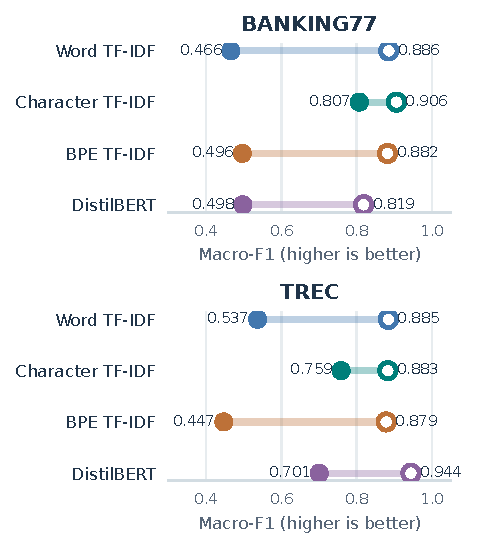
\includegraphics[width=\linewidth]{performance_overview.pdf}
  \caption{The main result at a glance. Filled points show averaged Macro-F1 at 20\% perturbation, hollow points show clean performance.}
  \label{fig:overview}
  \vspace{1 mm}
\end{figure}



\minisection{Performance across the full attack-strength range}
Figure~\ref{fig:robustness} follows all measured strengths. Mean Macro-F1 decreases and attack success rises as more eligible positions are changed. Character features lead on BANKING77 throughout. On TREC, DistilBERT leads at 5\% (0.865 versus 0.853); character features lead from 10\% to 40\%, but DistilBERT leads again at 75\% (0.411 versus 0.337). All four models are evaluated through 75\%.

\begin{figure}[H]
\centering
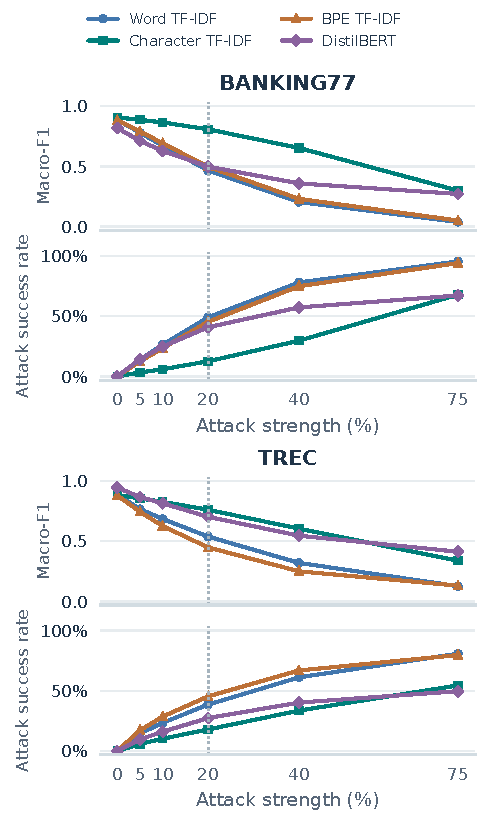
\includegraphics[width=\linewidth]{attack_strength_overview.pdf}
\caption{Macro-F1 (higher is better) and attack success rate (lower is better), averaged equally across four effective families. Zero denotes clean text; the dotted line marks 20\%.}
\label{fig:robustness}
\end{figure}

\minisection{What remains at 40\% and 75\%?}
The stronger attacks reveal substantial losses even for the most robust representation (Figure~\ref{fig:strong-attacks}).
On BANKING77, character Macro-F1 falls from 0.653 at 40\% to 0.299 at 75\%, while word and BPE features reach 0.039 and 0.051. DistilBERT reaches 0.271. At 75\%, attacks overturn 67.8\% of the predictions that the character model got right when clean.

On TREC, character Macro-F1 falls from 0.603 at 40\% to 0.337 at 75\%, while word and BPE features reach 0.126 and 0.130. DistilBERT reaches 0.411. At 75\%, attacks overturn 54.4\% of the predictions that the character model got right when clean.


\begin{figure}[H]
\centering
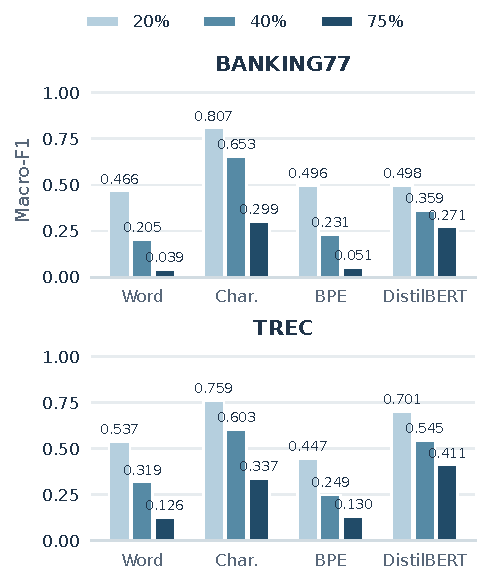
\includegraphics[width=\linewidth]{strong_attack_comparison.pdf}
\caption{Mean Macro-F1 at 20\%, 40\% and 75\%, using the same four-family average.}
\label{fig:strong-attacks}
\end{figure}

\minisection{The attack family changes the trajectory}
The family breakdown in Figure~\ref{fig:families} explains why the mean alone is incomplete. DistilBERT stays at its clean score under the tested invisible controls through 75\%, while its BANKING77 Macro-F1 heavily suffers under compatibility substitutions . Its preprocessing discards the tested invisible characters. Character features also degrade: compatibility substitutions give them the lowest 75\% score on both datasets. Mixed attacks sample applicable transformations and as such will not necessarily perform like the worst single family.

\begin{figure}[H]
\centering
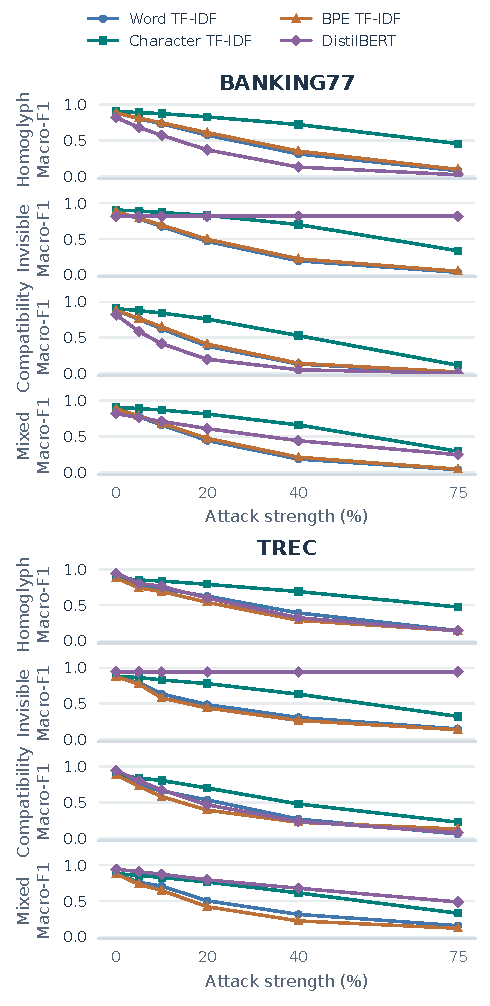
\includegraphics[width=\linewidth]{attack_strength_by_family.pdf}
\caption{Macro-F1 by attack family and dataset across all available strengths. Each curve begins at its clean score. Composition is omitted because it changes no test inputs. All four models cover the full range through 75\%.}
\label{fig:families}
\end{figure}

\Needspace{0.7\textheight}
\minisection{How much of the lost score is recovered?}

\begin{figure}[H]
\centering
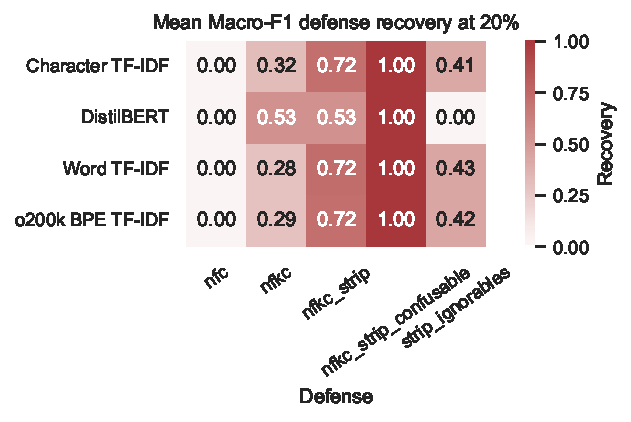
\includegraphics[width=\linewidth]{defense_recovery.pdf}
\caption{Macro-F1 before and after repair, averaged across the four effective families at 20\%. Full repair nearly reaches the clean baseline; its map covers the restricted attack whitelist.}
\label{fig:defense}
\end{figure}


\begin{table*}[!tbp]
\centering\small
\caption{Mean defense recovery at 20\% strength, shown as \(100R\): 72.31 means 72.31\% of the lost score recovered on the equal-family average. Each classical row averages four defined family ratios. DistilBERT averages three, excluding invisible attacks because their raw score loss is zero. Rounded 100.00 values need not imply exact recovery.}
\begin{tabular}{@{}lrrrrr@{}}
\toprule
\tabhead Model & NFC & NFKC & Removal & NFKC + removal & Full repair \\
\midrule
\multicolumn{6}{l}{\textbf{BANKING77}} \\
Word TF-IDF & 0.00 & 28.66 & 42.96 & 72.31 & 99.98 \\
Character TF-IDF & 0.00 & 31.00 & 42.67 & 72.29 & 100.00 \\
BPE TF-IDF & 0.00 & 29.18 & 43.13 & 72.43 & 99.98 \\
DistilBERT & 0.00 & 54.42 & 0.00 & 54.42 & 99.99 \\
\addlinespace[5pt]
\multicolumn{6}{l}{\textbf{TREC}} \\
Word TF-IDF & 0.00 & 28.17 & 42.67 & 72.06 & 100.00 \\
Character TF-IDF & 0.00 & 32.28 & 40.21 & 70.86 & 100.00 \\
BPE TF-IDF & 0.00 & 28.27 & 41.63 & 70.98 & 99.99 \\
DistilBERT & 0.00 & 51.97 & 0.00 & 51.97 & 100.00 \\
\bottomrule
\end{tabular}

\label{tab:defense-recovery}
\end{table*}

Combining NFKC and control removal improves classical recovery because they repair different families. DistilBERT already discards the tested controls, so removal adds nothing. Its combined recovery is 54.42\% on BANKING77 and 51.97\% on TREC over three attack families (not the homoglyph).

\minisection{A worked recovery calculation}
\label{sec:recovery-example}
For BANKING77 word TF--IDF under the 20\% mixed attack, clean Macro-F1 is 0.885686, raw attacked Macro-F1 is 0.441687, and NFKC plus removal raises it to 0.837951. Applying Equation~\ref{eq:recovery} gives:
\begin{equation*}
R_{\mathrm{mixed}}=\frac{0.837951-0.441687}{0.885686-0.441687}\approx 0.892.
\end{equation*}

The defense recovers 89.2\% of this loss. Its four-family mean is 72.31\%: compatibility and invisible attacks are fully repaired, while homoglyphs are not. Calculating \(R\) from cross-family average scores would weight families by their initial loss; the table instead averages their recovery ratios equally.
 Near-complete recovery is measured on this restricted attack set.
\section{Tokenization and Failure}

For both \texttt{o200k\_base} and DistilBERT WordPiece, we compare clean and attacked token sequences using relative token-count change, normalized token edit distance, and multiset Jaccard overlap. The principal association model is a binomial regression restricted to clean-correct, effectively changed examples:
\begin{equation}
\mathrm{logit}\,P(\mathrm{failure}) = \beta_0 + \beta_1 d_{\mathrm{tok}} + \beta_2 \Delta n + \mathbf{c},
\end{equation}
where $\mathbf{c}$ controls for dataset, attack family, strength, and model seed when applicable. Standard errors are clustered by original example because each input appears under repeated perturbations. Coefficients are interpreted as associations, not causal effects.

The association is large for both subword systems. For BPE features, a one-standard-deviation increase in normalized token edit distance corresponds to 2.64 times the odds of failure (95\% CI 2.46--2.82). For DistilBERT WordPiece the odds ratio is 3.61 (3.38--3.85). Relative token-count change remains positively associated with BPE failure (OR 1.25, 1.19--1.32) after controlling for edit distance, but its DistilBERT coefficient is slightly negative (OR 0.94, 0.91--0.97). This sign difference cautions against using token count alone as a robustness proxy: the identity and ordering of replacement tokens contain information not captured by length.

Figure~\ref{fig:tokenization} provides a nonparametric view. Failure rates rise across token-edit quartiles for both datasets and systems, consistent with the regression. The analysis is restricted to clean-correct examples with at least one effective code-point change, so it models attack failure rather than conflating it with baseline errors. Nevertheless, the result is associational. Attack families jointly determine both token disruption and difficulty, and the controls cannot establish that tokenization changes themselves cause each error.

\begin{figure}[t]
  \centering
  \IfFileExists{../artifacts/figures/token_disruption_failure.pdf}{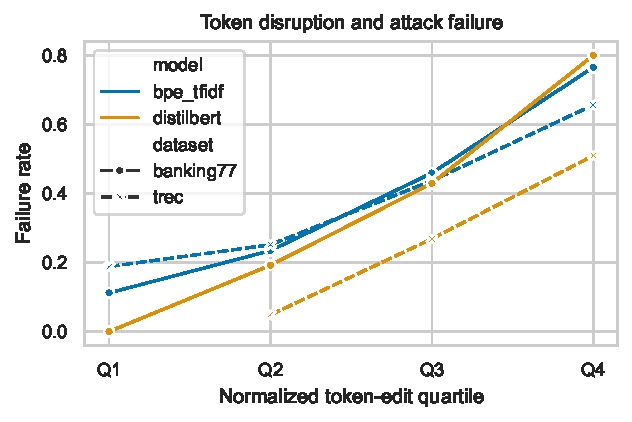
\includegraphics[width=\columnwidth]{token_disruption_failure.pdf}}{\fbox{Tokenization figure pending.}}
  \caption{Failure rate by token-sequence disruption quartile.}
  \label{fig:tokenization}
\end{figure}

\subsection{Two examples behind the scores}
I selected as an example 2 dataset/model pair with very mixed-attack ASR at 20\%, then looked at its attacks across families. The largest successful probability loss (resulting in missclassification) and largest repair gain identify the same sentence, shown in (Table~\ref{tab:example1}). The second example instead has the largest loss among resisted attacks(so correct classification even under attack) (Table~\ref{tab:example2}).

The gt-probability is the probability assigned to the ground truth (gt) label.

\begin{table*}[t]
\centering
\scriptsize
\caption{Rule-selected examples; non-ASCII and invisible code points are shown explicitly.}
\begin{tabularx}{\textwidth}{@{}llllX@{}}
\toprule
Case & Dataset & Model & Attack & Auditable text \\
\midrule
Successful attack & BANKING77 & Word TF-IDF & homoglyph & clean: There is a suspicious direct debit payment.; attacked: T[U+04BB]ere is a suspi[U+0441][U+0456]ous dire[U+0441]t deb[U+0456]t payment. \\
Recovered by defense & BANKING77 & Word TF-IDF & homoglyph & clean: There is a suspicious direct debit payment.; attacked: T[U+04BB]ere is a suspi[U+0441][U+0456]ous dire[U+0441]t deb[U+0456]t payment. \\
Prediction resisted & BANKING77 & Word TF-IDF & invisible & clean: Do you offer Visa or Mastercard?; attacked: Do yo[U+200B]u of[U+200B]fer Vi[U+200D]s[U+2060]a or Mastercar[U+200B]d? \\
\bottomrule
\end{tabularx}
\label{tab:errors}
\end{table*}


Lookalikes overturn the first prediction; repair restores it. In the second case, confidence falls but the correct label stays first. Every non-ASCII code point is exposed in the audit string as they would be indistinguishable (else there would be no point in this whole study).

\subsection{Discussion}
The main takeaway that can be taken from these experiments is that good performance on clean text can hide a dependence on its exact spelling and encoding. Character features generally tolerate the tested changes better than word and BPE features, probably because of their higher "density" but they still struggle when much of the input is modified. DistilBERT also shows how different the outcome can depend on the attack: its preprocessing removes the tested invisible characters, while other substitutions remain damaging. A single average score would hide these differences.

The defense results show how much can be recovered by changing the way the input is handled, without retraining the classifier. This makes simple preprocessing worth considering before moving to a more complex model. The almost complete recovery with full repair needs some caution, though: the repair map covers the characters used by the attacks. I would expect a less complete result with unfamiliar substitutions, and this experiment cannot tell us how safely the same rules would handle legitimate Unicode text in other languages, some possible next steps may be the study of smarter, less destructive and/or more generalized defenses for homoglyphs attacks.

Jev changes very little under these attacks, even when the local models lose much of their performance. The uncertainty is mainly about why it behaves this way and how far that behavior would generalize. Unknown training data, possible exposure to the datasets, and any preprocessing behind the API make it difficult to attribute the result to the model's architecture. Normalization similar to the defenses used here could explain part of its robustness, but I have no evidence that the API applies it. The experiment measures the behavior of the service as a whole.


\section{Statement on the Use of Generative AI}

ChatGPT and Codex were used to brainstorm and refine the project design; locate and cross-check primary literature, dataset cards, Unicode standards, and software documentation; scaffold and review the Jupyter notebooks and LaTeX report; assist with debugging, plotting, statistical checks, and proofreading; and document reproducibility steps. No paid model API was used in the experiments. The student remained responsible for running the experiments, checking citations against primary sources, inspecting generated examples and results, evaluating whether interpretations were supported, and approving the final submitted report and code.



\begingroup
\small
\bibliographystyle{plainnat}
\bibliography{references}
\endgroup
\end{document}
